In Exercises \ref{sinecosinegraphfirst} - \ref{sinecosinegraphlast}, graph one cycle of the given function.  State the period, amplitude, phase shift and vertical shift of the function.

\begin{multicols}{3}

\begin{enumerate}

\item $f(t) = 3\sin(t)$ \label{sinecosinegraphfirst}
\item $g(t) = \sin(3t)$
\item $h(t)  = -2\cos(t)$

\setcounter{HW}{\value{enumi}}

\end{enumerate}

\end{multicols}

\begin{multicols}{3}

\begin{enumerate}

\setcounter{enumi}{\value{HW}}

\item $f(t)  = \cos \left( t - \frac{\pi}{2} \right)$
\item $g(t)  = -\sin \left( t + \frac{\pi}{3} \right)$
\item $h(t) = \sin(2t - \pi)$ \vphantom{$\left( \frac{\pi}{2} \right)$}

\setcounter{HW}{\value{enumi}}

\end{enumerate}

\end{multicols}

\begin{multicols}{3}

\begin{enumerate}

\setcounter{enumi}{\value{HW}}

\item $f(t)  = -\frac{1}{3}\cos \left( \frac{1}{2}t + \frac{\pi}{3} \right)$
\item $g(t) = \cos (3t - 2\pi) + 4$ \vphantom{$\left( \frac{1\pi}{2} \right)$}
\item $h(t)  = \sin \left( -t - \frac{\pi}{4} \right) - 2$ \vphantom{$\left( \frac{1\pi}{2} \right)$}

\setcounter{HW}{\value{enumi}}

\end{enumerate}

\end{multicols}

\begin{multicols}{3}

\begin{enumerate}

\setcounter{enumi}{\value{HW}}

\item $f(t) = \frac{2}{3} \cos \left( \frac{\pi}{2} - 4t \right) + 1$
\item $g(t) = -\frac{3}{2} \cos \left( 2t + \frac{\pi}{3} \right) - \frac{1}{2}$
\item $h(t) = 4\sin (-2\pi t + \pi)$ \vphantom{$\left( \frac{1\pi}{2} \right)$}  \label{sinecosinegraphlast}

\setcounter{HW}{\value{enumi}}

\end{enumerate}

\end{multicols}

In Exercises \ref{fitsinecosinefirst} - \ref{fitsinecosinelast},  a sinusoid is graphed. Find a formula for the sinusoid in the form $S(t) = A \sin(\omega t + \phi) + B$ and $C(t) = A \cos(\omega t + \phi) + B$.  Select $\omega$ so  $\omega > 0$. Check your answer by graphing.

\begin{multicols}{2}
\begin{enumerate}
\setcounter{enumi}{\value{HW}}

\item $~$   \label{fitsinecosinefirst}  %$S(t) = 4 \sin \left(t + \frac{\pi}{4} \right)$, $C(t) = 4 \cos \left(t - \frac{\pi}{4} \right)$

\begin{mfpic}[16]{-5}{5}{-5}{5}
\tlabel[cc](5,-0.30){\scriptsize $t$}
\tlabel[cc](0.25,5){\scriptsize $y$}
\axes
\xmarks{-4 step 1 until 4}
\ymarks{-4 step 1 until 4}
\point[4pt]{(-3.927, 0), (-2.356, -4), (-0.7854, 0), (0.7854, 4), (2.356, 0)}
\tlabel[cc](-3, 0.5){ \scriptsize $\left( -\frac{5\pi}{4}, 0 \right)$}
\tlabel[cc](-2.356, -4.5){ \scriptsize $\left( -\frac{3\pi}{4}, -4 \right)$}
\gclear \tlabelrect(0.25, -0.6){ \scriptsize $\left( -\frac{\pi}{4}, 0 \right)$ \vphantom{$\dfrac{5}{2}$}}
\tlabel[cc](0.9, 4.5){\scriptsize $\left( \frac{\pi}{4}, 4 \right)$}
\tlabel[cc](3.25, 0.5){ \scriptsize $\left( \frac{3\pi}{4}, 4 \right)$}
\tlpointsep{4pt}
%\axislabels {x}{{$\frac{\pi}{2}$} 1.5708, {$\pi$} 3.1416, {$\frac{3\pi}{2}$} 4.7124, {$2\pi$} 6.2832}
%\axislabels {y}{{$-3$} -3, {$3$} 3}
\penwd{1.25pt}
\arrow \reverse \arrow \function{-5, 5,  0.1}{4*sin(x+(pi/4))}
\end{mfpic}   


\item$~$     % $S(t) = -3 \sin(t) + 3$, $C(t) = -3 \cos\left(t - \frac{\pi}{2}\right) + 3$

\begin{mfpic}[16]{-6}{6}{-1}{9}
\tlabel[cc](6,-0.30){\scriptsize $t$}
\tlabel[cc](0.25,9){\scriptsize $y$}
\axes
\xmarks{-5 step 1 until 5}
\ymarks{1 step 1 until 8}
\point[4pt]{(-4.712, 0), (-1.571, 6), (0,3), (1.571, 0), (4.712, 6)}
\tlabel[cc](-4.712, -0.75){\scriptsize $\left( -\frac{3\pi}{2}, 0 \right)$}
\tlabel[cc](-1.571, 6.5){\scriptsize $\left( -\frac{\pi}{2}, 6 \right)$}
\tlabel[cc](0.75, 3){ \scriptsize $\left(0, 3 \right)$}
\tlabel[cc](4.712, 6.5){\scriptsize $\left( \frac{3 \pi}{2}, 6 \right)$}
\tlabel[cc](1.571, -0.75){\scriptsize $\left( \frac{\pi}{2}, 0 \right)$}
\tlpointsep{4pt}
%\axislabels {x}{{$\frac{\pi}{2}$} 1.5708, {$\pi$} 3.1416, {$\frac{3\pi}{2}$} 4.7124, {$2\pi$} 6.2832}
%\axislabels {y}{{$-3$} -3, {$3$} 3}
\penwd{1.25pt}
\arrow \reverse \arrow \function{-6, 6,  0.1}{3- 3*sin(x)}
\end{mfpic}  

\setcounter{HW}{\value{enumi}}
\end{enumerate}
\end{multicols}

\begin{multicols}{2}
\begin{enumerate}
\setcounter{enumi}{\value{HW}}

\item $~$    %$S(t) = 3 \sin \left( 2t - \frac{\pi}{3} \right)$, $C(t) = 3 \cos \left( 2t - \frac{5\pi}{6} \right)$

\begin{mfpic}[15]{-6}{6}{-5}{5}
\tlabel[cc](6,-0.30){\scriptsize $t$}
\tlabel[cc](0.25,5){\scriptsize $y$}
\axes
\xmarks{-5 step 1 until 5}
\ymarks{-4 step 1 until 4}
\point[4pt]{(-4.974, 3), (-4.189, 0), (-3.403, -3), (-2.618, 0), (-1.832, 3), (-1.047, 0), (-0.2618, -3), (0.5236, 0), (1.309, 3), (2.094, 0), (2.8880, -3), (3.665, 0), (4.45, 3), (5.236, 0)}
\tlabel[cc](-4.974, 3.75){ \scriptsize $\left( -\frac{19 \pi}{12}, 3 \right)$}
\tlabel[cc](-3.403, -3.75){ \scriptsize $\left( -\frac{13 \pi}{12}, -3 \right)$}
\tlabel[cc] (-1.832, 3.75){ \scriptsize $\left( -\frac{7 \pi}{12}, 3 \right)$}
\gclear \tlabelrect(0, -3.75){ \scriptsize $\left( -\frac{\pi}{12}, -3 \right)$}
\tlabel[cc] (1.309, 3.75){ \scriptsize $\left( \frac{5 \pi}{12}, 3 \right)$}
\tlabel[cc](2.880, -3.75){ \scriptsize $\left( \frac{11 \pi}{12}, -3 \right)$}
\tlabel[cc] (4.45, 3.75){ \scriptsize $\left( \frac{17 \pi}{12}, 3 \right)$}

\tlpointsep{4pt}
%\axislabels {x}{{$\frac{\pi}{2}$} 1.5708, {$\pi$} 3.1416, {$\frac{3\pi}{2}$} 4.7124, {$2\pi$} 6.2832}
%\axislabels {y}{{$-3$} -3, {$3$} 3}
\penwd{1.25pt}
\arrow \reverse \arrow \function{-6, 5.5,  0.1}{3*sin((2*x)-(pi/3))}
\end{mfpic}   


\item$~$     \label{fitsinecosinelast}  % $S(t) =  \frac{7}{2} \sin(\pi t) + \frac{1}{2}$, $C(t) = \frac{7}{2} \cos\left(\pi t \frac{\pi}{2} \right) + \frac{1}{2}$

\begin{mfpic}[22][15]{-5}{5}{-5}{5}
\tlabel[cc](5,-0.30){\scriptsize $t$}
\tlabel[cc](0.25,5){\scriptsize $y$}
\axes
\xmarks{-4 step 1 until 4}
\ymarks{-4 step 1 until 4}
\point[4pt]{ (-4, 0.5), (-3.5, 4), (-3, 0.5), (-2.5, -3), (-2, 0.5), (-1.5, 4), (-1, 0.5), (-0.5, -3), (0, 0.5), (0.5, 4), (1, 0.5), (1.5,-3), (2, 0.5), (2.5,4), (3, 0.5), (3.5,-3), (4, 0.5) }
%\tlabel[cc](-4.5, -3.5){\scriptsize $(-4.5, -3)$}
\tlabel[cc](-3.5, 4.5){\scriptsize $(-3.5, 4)$}
\tlabel[cc](-2.5, -3.5){\scriptsize $(-2.5, -3)$}
\tlabel[cc](-1.5, 4.5){\scriptsize $(-1.5, 4)$}
%\tlabel[cc](-0.5, -3.5){\scriptsize $(-0.5, -3)$}
\gclear \tlabelrect(0.75, 4.5){\scriptsize $(0.5, 4)$}
\tlabel[cc](1.5, -3.5){\scriptsize $(1.5, -3)$}
\tlabel[cc](2.5, 4.5){\scriptsize $(2.5, 4)$}
%\tlabel[cc](2.5, -3.5){\scriptsize $(2.5, -3)$}
%\tlabel[cc](4.5, 4.5){\scriptsize $(4.5, 4)$}

\tlpointsep{4pt}
%\axislabels {x}{{$\frac{\pi}{2}$} 1.5708, {$\pi$} 3.1416, {$\frac{3\pi}{2}$} 4.7124, {$2\pi$} 6.2832}
%\axislabels {y}{{$-3$} -3, {$3$} 3}
\penwd{1.25pt}
\arrow \reverse \arrow \function{-4.25, 4.25,  0.1}{(3.5*sin(pi*x))+0.5}
\end{mfpic}   

\setcounter{HW}{\value{enumi}}
\end{enumerate}
\end{multicols}


\begin{enumerate}
\setcounter{enumi}{\value{HW}}

\item  Use the graph of  $S(t) = 4 \sin(t)$ to graph each of the following functions. State the period of each.

\begin{multicols}{2}

\begin{enumerate}

\item $f(t) = | 4 \sin(t)|$

\item $g(t) = \sqrt{4 \sin(t)}$

\end{enumerate}
\end{multicols}


\setcounter{HW}{\value{enumi}}
\end{enumerate}

In Exercises \ref{exploregraphsfirst} - \ref{exploregraphslast}, use a graphing utility to graph each function and discuss the related questions with your classmates.


\begin{enumerate}

\setcounter{enumi}{\value{HW}}

\item  $f(t) = \cos(3t) + \sin(t)$.  Is this function periodic?  If so, what is the period? \label{exploregraphsfirst}
\item  $f(t) = \frac{\sin(t)}{t}$.  What appears to be the horizontal asymptote of the graph? 
\item  $f(t) = t \sin(t)$.  Graph $y = \pm t$. What do you notice? 
\item  $f(t) = \sin\left(\frac{1}{t}\right)$.  What's happening as $t \rightarrow 0$?
%\item  $f(x) = x - \tan(x)$.  Graph $y = x$ on the same set of axes and describe the behavior of $f$.  
\item  $f(t) = e^{-0.1t} \left( \cos(2t) + \sin(2t)\right)$.  Graph $y = \pm e^{-0.1t}$ on the same set of axes. What do you notice?
\item  $f(t) = e^{-0.1t} \left( \cos(2t) + 2\sin(t)\right)$.  Graph $y = \pm e^{-0.1t}$ on the same set of axes.  What do you notice? \label{exploregraphslast}

\setcounter{HW}{\value{enumi}}

\end{enumerate}

\begin{enumerate}

\setcounter{enumi}{\value{HW}}

\item Show every constant function $f$ is periodic by explaining why $f(x + 117) = f(x)$ for all real numbers $x$. Then show that $f$ has no period by showing that you cannot find a \emph{smallest} number $p$ such that $f(x + p) = f(x)$ for all real numbers $x$.  

\smallskip

Said differently, show that $f(x + p) = f(x)$ for all real numbers $x$ for ALL values of $p > 0$, so no smallest value exists to satisfy the definition of `period'.

\setcounter{HW}{\value{enumi}}

\end{enumerate}

\begin{enumerate}

\setcounter{enumi}{\value{HW}}

\item  The sounds we hear are made up of mechanical waves.  The note `A' above the note `middle C' is a sound wave with ordinary frequency $f = 440$ Hertz $= 440 \frac{\text{cycles}}{\text{second}}$.  Find a sinusoid which models this note, assuming that the amplitude is $1$ and the phase shift is $0$.

\item The voltage $V$ in an alternating current source has amplitude $220 \sqrt{2}$ and ordinary frequency $f = 60$ Hertz.  Find a sinusoid which models this voltage.  Assume that the phase is $0$.


\item \label{heightlondoneye} The \href{http://en.wikipedia.org/wiki/London_Eye}{\underline{London Eye}} is a popular tourist attraction in London, England and is one of the largest Ferris Wheels in the world.  It has a diameter of 135 meters and makes one revolution (counter-clockwise) every 30 minutes.  It is constructed so that the lowest part of the Eye reaches ground level, enabling passengers to simply walk on to, and off of, the ride.  Find a sinsuoid which models the height $h$ of the passenger above the ground in meters $t$ minutes after they board the Eye at ground level.

\item \label{leftrightlondoneye} On page \pageref{equationsforcircularmotion} in Section \ref{cosinesinebeyond}, we found the $x$-coordinate of counter-clockwise motion on a circle of radius $r$ with angular frequency $\omega$ to be $x = r\cos(\omega t)$, where $t=0$ corresponds to the point $(r,0)$.  Suppose we are in the situation of Exercise \ref{heightlondoneye} above.  Find a sinsusoid which models the horizontal \textit{displacement} $x$ of the passenger from the center of the Eye in meters $t$ minutes after they board the Eye.  Here we take $x(t) > 0$ to mean the passenger is to the \textit{right} of the center, while $x(t) < 0$ means the passenger is to the \textit{left} of the center.

\item  In Exercise \ref{yoyotrick} in Section \ref{RadianMeasure}, we introduced the yo-yo trick `Around the World' in which a yo-yo is thrown so it sweeps out a vertical circle.  As in that exercise, suppose the yo-yo string is 28 inches and it completes one revolution in 3 seconds.  If the closest the yo-yo ever gets to the ground is 2 inches, find a sinsuoid which models the height $h$ of the yo-yo above the ground in inches $t$ seconds after it leaves its lowest point.



\item  Consider the pendulum below.  Ignoring air resistance, the angular displacement of the pendulum from the vertical position, $\theta$, can be modeled as a sinusoid.\footnote{Provided $\theta$ is kept `small.'  Carl remembers the `Rule of Thumb' as being $20^{\circ}$ or less.  Check with your friendly neighborhood physicist to make sure.}


\begin{center}

\begin{mfpic}[15]{-3}{3}{-5}{1}
\polyline{(0,0), (0,-5)}
\dashed \polyline{(0,0), (2.5, -4.33)}
\arrow \parafcn{275, 295, 5}{4*dir(t)}
\tlabel[cc](1.29, -4.83){$\theta$}
\hatchcolor[gray]{.7}
\lhatch \rect{(-3,0), (3,1)}
\fillcolor[gray]{.7} 
\gfill \circle{(0,-5),0.25}
\gfill \circle{(2.5, -4.33),0.20}
\penwd{1.025}
\circle{(0,-5),0.25}
\circle{(2.5, -4.33),0.25}
\rect{(-3,0), (3,1)}
\end{mfpic} 
\end{center}

The amplitude of the sinusoid is the same as the initial angular displacement, $\theta_{\text{\tiny $0$}}$, of the pendulum and the  period of the motion is given by

\[T = 2\pi \sqrt{\dfrac{\ell}{g}}\]

where $\ell$ is the length of the pendulum and $g$ is the acceleration due to gravity.

\begin{enumerate}

\item  Find a sinusoid which gives the angular displacement $\theta$ as a function of time, $t$. Arrange things so $\theta(0) = \theta_{\text{\tiny $0$}}$.

\item  In Exercise \ref{pendulumproblem} section \ref{RootRadicalFunctions}, you found the length of the pendulum needed in Jeff's antique Seth-Thomas clock to ensure the period of the pendulum is $\frac{1}{2}$ of a second. Assuming the initial displacement of the pendulum is $15^{\circ}$, find a sinusoid which models the displacement of the pendulum $\theta$ as a function of time, $t$, in seconds. 

\end{enumerate}

\newpage

\item  The table below lists the average temperature of Lake Erie as measured in Cleveland, Ohio on the first of the month for each month during the years 1971 -- 2000.\footnote{See this website: \href{http://www.erh.noaa.gov/cle/climate/cle/normals/laketempcle.html}{\underline{http://www.erh.noaa.gov/cle/climate/cle/normals/laketempcle.html}.}}  For example,   $t=3$ represents the average of the temperatures recorded for Lake Erie on every March 1 for the years 1971 -- 2000.

\medskip

\small

\noindent \begin{tabular}{|l|r|r|r|r|r|r|r|r|r|r|r|r|} \hline
Month  & & & & & & & & & & & & \\
Number, $t$ & 1 & 2 & 3 & 4 & 5 & 6 & 7 & 8 & 9 & 10 & 11 & 12\\ 
\hline 
Temperature  & & & & & & & & & & & & \\
($^{\circ}$ F), $T$ & 36 & 33 & 34 & 38 & 47 & 57 & 67 & 74 & 73 & 67 & 56 & 46 \\ \hline
\end{tabular}

\normalsize

\medskip

\begin{enumerate}

\item \label{LakeErieTempData} Using the techniques discussed in Example \ref{sinusoidsunlight}, fit a sinusoid to these data. 

\item  Graph your model along with the data set to judge the reasonableness of the fit.

\item Use the model from \ref{LakeErieTempData} to predict the average temperature recorded for Lake Erie on April $15^{\text{th}}$ and September $15^{\text{th}}$ during the years 1971--2000.\footnote{The computed average is $41^{\circ}$F for April $15^{\text{th}}$ and $71^{\circ}$F for September $15^{\text{th}}$.}

\item Compare your results to those obtained using a graphing utility.

\end{enumerate}

\item  The fraction of the moon illuminated at midnight Eastern Standard Time on the $t^{\text{th}}$ day of June, 2009 is given in the table below.\footnote{See this website: \href{http://www.usno.navy.mil/USNO/astronomical-applications/data-services/frac-moon-ill}{\underline{http://www.usno.navy.mil/USNO/astronomical-applications/data-services/frac-moon-ill}.}} 


\medskip

\small

\noindent \begin{tabular}{|l|r|r|r|r|r|r|r|r|r|r|} \hline
Day of  & & & & & & & & & & \\
June, $t$ & 3 & 6 & 9 & 12 & 15 & 18 & 21 & 24 & 27 & 30\\ 
\hline 
Fraction  & & & & & & & & & & \\
Illuminated, $F$ & 0.81 & 0.98 & 0.98 & 0.83 & 0.57 & 0.27 & 0.04 & 0.03 & 0.26 & 0.58  \\ \hline
\end{tabular}

\normalsize

\medskip

\begin{enumerate}

\item \label{MoonIllumination} Using the techniques discussed in Example \ref{sinusoidsunlight}, fit a sinusoid to these data.\footnote{You may want to plot the data before you find the phase shift.} 

\item  Graph your model along with the data set to judge the reasonableness of the fit.

\item Use the model from \ref{MoonIllumination} to predict the fraction of the moon illuminated on June 1, 2009. \footnote{The listed fraction is $0.62$.}

\item Compare your results to those obtained using a graphing utility.

\end{enumerate}


\item \label{graphdesmosregression}  Use a graphing utility to graph $y = 8.36 \sin(-294.81t  - 26.53) + 12.06$.  (This is the regression model produced by desmos in Example \ref{sinusoidsunlight}.) Zoom in, as needed, until you start to see the wave-like nature of the graph.  Use Theorem \ref{sinusoidform} to determine a window which produces exactly one complete cycle of this sinusoid and check your answer graphically.

\item   \label{proofsinusoidformexercise} Use Theorem \ref{transformationsthm} to prove Theorem \ref{sinusoidform}.


\item  With the help of your classmates, research \href{http://en.wikipedia.org/wiki/Amplitude_modulation}{\underline{Amplitude Modulation}} and \href{http://en.wikipedia.org/wiki/Frequency_modulation}{\underline{Frequency Modulation}}.

\item What other things in the world might be roughly sinusoidal?  Look to see what models you can find for them and share your results with your class.

\end{enumerate}

\newpage


\subsection{Answers}

\begin{enumerate}

\item \begin{multicols}{2} \raggedcolumns
$f(t) = 3\sin(t)$\\
Period: $2\pi$\\
Amplitude: $3$\\
Phase Shift: $0$\\
Vertical Shift: $0$\\

\begin{mfpic}[25][15]{-0.25}{7}{-3.5}{3.75}
\point[4pt]{(0,0), (1.5708,3), (3.1416, 0), (4.7124,-3), (6.2832,0)}
\axes
\tlabel[cc](7,-0.30){$t$}
\tlabel[cc](0.25,3.75){$y$}
\xmarks{1.5708, 3.1416, 4.7124, 6.2832 }
\ymarks{-3,3}
\tlpointsep{4pt}
\axislabels {x}{{$\frac{\pi}{2}$} 1.5708, {$\pi$} 3.1416, {$\frac{3\pi}{2}$} 4.7124, {$2\pi$} 6.2832}
\axislabels {y}{{$-3$} -3, {$3$} 3}
\penwd{1.25pt}
\function{0, 6.2832, 0.1}{3*sin(x)}
\end{mfpic}

\end{multicols}

\item \begin{multicols}{2} \raggedcolumns
$g(t)  = \sin(3t)$\\
Period: $\frac{2\pi}{3}$\\
Amplitude: $1$\\
Phase Shift: $0$\\
Vertical Shift: $0$\\

\begin{mfpic}[70][50]{-0.25}{2.5}{-1.25}{1.25}
\point[4pt]{(0,0), (0.5236,1), (1.0472,0), (1.5708,-1), (2.0944,0)}
\axes
\tlabel[cc](2.5,-0.15){$t$}
\tlabel[cc](0.15,1.25){$y$}
\xmarks{0.5236, 1.0472, 1.5708, 2.0944}
\ymarks{-1,1}
\tlpointsep{4pt}
\axislabels {x}{{$\frac{\pi}{6}$} 0.5236, {$\frac{\pi}{3}$} 1.0472, {$\frac{\pi}{2}$} 1.5708, {$\frac{2\pi}{3}$} 2.0944}
\axislabels {y}{{$-1$} -1, {$1$} 1}
\penwd{1.25pt}
\function{0, 2.0944, 0.1}{sin(3*x)}
\end{mfpic}

\end{multicols}

\item \begin{multicols}{2} \raggedcolumns
$h(t) = -2\cos(t)$\\
Period: $2\pi$\\
Amplitude: $2$\\
Phase Shift: $0$\\
Vertical Shift: $0$\\

\begin{mfpic}[25]{-0.25}{7}{-2.5}{2.5}
\point[4pt]{(0,-2), (1.5708,0), (3.1416, 2), (4.7124,0), (6.2832,-2)}
\axes
\tlabel[cc](7,-0.25){$t$}
\tlabel[cc](0.25,2.5){$y$}
\xmarks{1.5708, 3.1416, 4.7124, 6.2832}
\ymarks{-2,2}
\tlpointsep{4pt}
\axislabels {x}{{$\frac{\pi}{2}$} 1.5708, {$\pi$} 3.1416, {$\frac{3\pi}{2}$} 4.7124, {$2\pi$} 6.2832}
\axislabels {y}{{$-2$} -2, {$2$} 2}
\penwd{1.25pt}
\function{0, 6.2832, 0.1}{-2*cos(x)}
\end{mfpic}

\end{multicols}

\item \begin{multicols}{2} \raggedcolumns
$f(t) = \cos \left( t - \frac{\pi}{2} \right)$\\
Period: $2\pi$\\
Amplitude: $1$\\
Phase Shift: $\frac{\pi}{2}$\\
Vertical Shift: $0$\\

\begin{mfpic}[22][40]{-0.25}{8.3}{-1.5}{1.5}
\point[4pt]{(1.5708,1), (3.1416, 0), (4.7124,-1), (6.2832,0), (7.854,1)}
\axes
\tlabel[cc](8.3,-0.25){$t$}
\tlabel[cc](0.25,1.5){$y$}
\xmarks{1.5708, 3.1416, 4.7124, 6.2832, 7.854}
\ymarks{-1,1}
\tlpointsep{4pt}
\axislabels {x}{{$\frac{\pi}{2}$} 1.5708, {$\pi$} 3.1416, {$\frac{3\pi}{2}$} 4.7124, {$2\pi$} 6.2832, {$\frac{5\pi}{2}$} 7.854}
\axislabels {y}{{$-1$} -1, {$1$} 1}
\penwd{1.25pt}
\function{1.5708, 7.854, 0.1}{cos(x - 1.5708)}
\end{mfpic}

\end{multicols}


\item \begin{multicols}{2} \raggedcolumns
$g(t) = -\sin \left( t + \frac{\pi}{3} \right)$\\
Period: $2\pi$\\
Amplitude: $1$\\
Phase Shift: $-\frac{\pi}{3}$\\
Vertical Shift: $0$\\

\begin{mfpic}[27][40]{-1.25}{5.75}{-1.5}{1.5}
\point[4pt]{(-1.0472,0), (0.5236,-1), (2.0944,0), (3.6652,1), (5.236,0)}
\axes
\tlabel[cc](5.75,-0.25){$t$}
\tlabel[cc](0.25,1.5){$y$}
\xmarks{-1.0472, 0.5236, 2.0944, 3.6652, 5.236}
\ymarks{-1,1}
\tlpointsep{4pt}
\axislabels {x}{{$-\frac{\pi}{3}$} -1.0472, {$\frac{\pi}{6}$} 0.5236, {$\frac{2\pi}{3}$} 2.0944, {$\frac{7\pi}{6}$} 3.6652, {$\frac{5\pi}{3}$} 5.236}
\axislabels {y}{{$-1$} -1, {$1$} 1}
\penwd{1.25pt}
\function{-1.0472, 5.236, 0.1}{-sin(x + 1.0472)}
\end{mfpic}

\end{multicols}

\item \begin{multicols}{2} \raggedcolumns
$h(t) = \sin(2t - \pi)$\\
Period: $\pi$\\
Amplitude: $1$\\
Phase Shift: $\frac{\pi}{2}$\\
Vertical Shift: $0$\\

\begin{mfpic}[35][50]{0}{5.25}{-1.15}{1.5}
\point[4pt]{(1.5708,0), (2.3562,1), (3.1415,0), (3.927,-1), (4.7124,0)}
\axes
\tlabel[cc](5.25,-0.25){$t$}
\tlabel[cc](0.25,1.5){$y$}
\xmarks{1.5708, 2.3562, 3.1415, 3.927, 4.7124}
\ymarks{-1,1}
\tlpointsep{4pt}
\axislabels {x}{{$\frac{\pi}{2}$} 1.5708, {$\frac{3\pi}{4}$} 2.3562, {$\pi$} 3.1415, {$\frac{5\pi}{4}$} 3.927, {$\frac{3\pi}{2}$} 4.7124}
\axislabels {y}{{$-1$} -1, {$1$} 1}
\penwd{1.25pt}
\function{1.5708, 4.7124, 0.1}{sin(2*x - 3.1415)}
\end{mfpic}

\end{multicols}

\item \begin{multicols}{2} \raggedcolumns
$f(t)  = -\frac{1}{3}\cos \left( \frac{1}{2}t  + \frac{\pi}{3} \right)$\\
Period: $4\pi$\\
Amplitude: $\frac{1}{3}$\\
Phase Shift: $-\frac{2\pi}{3}$\\
Vertical Shift: $0$\\

\begin{mfpic}[14][100]{-2.25}{11.5}{-0.5}{0.5}
\point[4pt]{(-2.0944, -0.3333), (1.0472, 0), (4.1888, 0.3333), (7.3304, 0), (10.472, -0.3333)}
\axes
\tlabel[cc](11.5,-0.05){$t$}
\tlabel[cc](0.25,0.5){$y$}
\xmarks{-2.0944, 1.0472, 4.1888, 7.3304, 10.472}
\ymarks{-0.3333, 0.3333}
\tlpointsep{4pt}
\axislabels {x}{{$-\frac{2\pi}{3}$} -2.0944, {$\frac{\pi}{3}$} 1.0472, {$\frac{4\pi}{3}$} 4.1888, {$\frac{7\pi}{3}$} 7.3304, {$\frac{10\pi}{3}$} 10.472}
\axislabels {y}{{$-\frac{1}{3}$} -0.3333, {$\frac{1}{3}$} 0.3333}
\penwd{1.25pt}
\function{-2.0944, 10.472, 0.1}{-0.3333*cos(0.5*x + 1.0472)}
\end{mfpic}

\end{multicols}

\item \begin{multicols}{2} \raggedcolumns
$g(t) = \cos (3t - 2\pi) + 4$\\
Period: $\frac{2\pi}{3}$\\
Amplitude: $1$\\
Phase Shift:  $\frac{2\pi}{3}$\\
Vertical Shift: 4\\

\begin{mfpic}[36][25]{-0.5}{5}{-0.5}{5.5}
\point[4pt]{(2.0944,5), (2.618,4), (3.1415,3), (3.6652,4), (4.1888,5)}
\axes
\tlabel[cc](5,-0.25){$t$}
\tlabel[cc](0.25,5.5){$y$}
\xmarks{2.0944, 2.618, 3.1415, 3.6652, 4.1888}
\ymarks{3,4,5}
\tlpointsep{4pt}
\axislabels {x}{{$\frac{2\pi}{3}$} 2.0944, {$\frac{5\pi}{6}$} 2.618, {$\pi$} 3.1415, {$\frac{7\pi}{6}$} 3.6652, {$\frac{4\pi}{3}$} 4.1888}
\axislabels {y}{{$3$} 3, {$4$} 4, {$5$} 5}
\penwd{1.25pt}
\function{2.0944, 4.1888, 0.1}{cos(3*x - 6.2834) + 4}
\end{mfpic}

\end{multicols}

\item \begin{multicols}{2} \raggedcolumns
$h(t) = \sin \left( -t - \frac{\pi}{4} \right) - 2$ \\
Period: $2\pi$\\
Amplitude: $1$\\
Phase Shift: $-\frac{\pi}{4}$ (You need to use \\ \vspace*{.1in}
$y = -\sin \left( t + \frac{\pi}{4} \right) - 2 $ to find this.)\footnote{Two cycles of the graph are shown to illustrate the discrepancy discussed on page \pageref{phaseshiftissue}.}\\
Vertical Shift: $-2$\\

\begin{mfpic}[13][27]{-7.5}{6.5}{-3.25}{0.5}
\point[4pt]{(-7.0686,-2), (-5.4979,-3), (-3.927,-2), (-2.3562,-1), (-0.7854,-2), (0.7854,-3), (2.3562,-2), (3.927,-1), (5.4979,-2)}
\axes
\tlabel[cc](6.5,-0.25){$t$}
\tlabel[cc](0.25,0.5){$y$}
\xmarks{-7.0686, -5.4979, -3.927, -2.3562,-0.7854, 0.7854, 2.3562, 3.927, 5.4979}
\ymarks{-3,-2,-1}
\tlpointsep{5pt}
\axislabels {x}{{$-\frac{9\pi}{4} \hspace{6pt}$} -7.0686, {$-\frac{7\pi}{4} \hspace{6pt}$} -5.4979, {$-\frac{5\pi}{4} \hspace{6pt}$} -3.927, {$-\frac{3\pi}{4} \hspace{6pt}$} -2.3562, {$-\frac{\pi}{4} \hspace{6pt}$} -0.7854, {$\frac{\pi}{4}$} 0.7854, {$\frac{3\pi}{4}$} 2.3562, {$\frac{5\pi}{4}$} 3.927, {$\frac{7\pi}{4}$} 5.4979}
\axislabels {y}{{$-3$} -3, {$-2$} -2, {$-1$} -1}
\penwd{1.25pt}
\function{-7.0686, 5.4979, 0.1}{-1*sin(x + 0.7854) - 2}
\end{mfpic}

\end{multicols}

\item \begin{multicols}{2} \raggedcolumns
$f(t) = \frac{2}{3} \cos \left( \frac{\pi}{2} - 4t \right) + 1$\\ 
Period: $\frac{\pi}{2}$\\
Amplitude: $\frac{2}{3}$\\ 
Phase Shift: $\frac{\pi}{8}$ (You need to use \\
$y = \frac{2}{3} \cos \left( 4t - \frac{\pi}{2} \right) + 1$ to find this.)\footnote{Again, we graph two cycles to illustrate the discrepancy discussed on page \pageref{phaseshiftissue}.}\\
Vertical Shift: $1$\\

\begin{mfpic}[52][45]{-1.5}{2.25}{-0.25}{2}
\point[4pt]{(-1.1781, 1.6667), (-0.7854, 1), (-0.3927, 0.3333), (0, 1), (0.3927, 1.6667), (0.7854, 1), (1.1781, 0.3333), (1.5708, 1), (1.9635, 1.6667)}
\axes
\tlabel[cc](2.25,-0.25){$t$}
\tlabel[cc](0.15,2){$y$}
\xmarks{-1.1781, -0.7854, -0.3927, 0.3927, 0.7854, 1.1781, 1.5708, 1.9635}
\ymarks{0.3333, 1, 1.6667}
\tlpointsep{4pt}
\axislabels {x}{{$-\frac{3\pi}{8} \hspace{6pt}$} -1.1781, {$-\frac{\pi}{4} \hspace{6pt}$} -0.7854, {$-\frac{\pi}{8} \hspace{6pt}$} -0.3927, {$\frac{\pi}{8}$} 0.3927, {$\frac{\pi}{4}$} 0.7854, {$\frac{3\pi}{8}$} 1.1781, {$\frac{\pi}{2}$} 1.5708, {$\frac{5\pi}{8}$} 1.9635}
\axislabels {y}{{$\frac{1}{3}$} 0.333, {$1$} 1, {$\frac{5}{3}$} 1.6667}
\penwd{1.25pt}
\function{-1.1781, 1.9635, 0.1}{0.6667*cos(4*x - 1.5708) + 1}
\end{mfpic}

\end{multicols}

\item \begin{multicols}{2} \raggedcolumns
$g(t)  = -\frac{3}{2} \cos \left( 2t + \frac{\pi}{3} \right) - \frac{1}{2}$\\
Period: $\pi$\\
Amplitude: $\frac{3}{2}$\\
Phase Shift: $-\frac{\pi}{6}$\\
Vertical Shift: $-\frac{1}{2}$\\

\begin{mfpic}[51][30]{-.75}{3}{-2.25}{1.5}
\point[4pt]{(-0.5236,-2), (0.2618,-0.5), (1.0472, 1), (1.8326, -0.5), (2.618, -2)}
\axes
\tlabel[cc](3,-0.25){$t$}
\tlabel[cc](0.15,1.5){$y$}
\xmarks{-0.5236, 0.2618, 1.0472, 1.8326, 2.618}
\ymarks{-2, -0.5, 1}
\tlpointsep{4pt}
\axislabels {x}{{$-\frac{\pi}{6}$} -0.5236, {$\frac{\pi}{12}$} 0.2618, {$\frac{\pi}{3}$} 1.0472, {$\frac{7\pi}{12}$} 1.8326, {$\frac{5\pi}{6}$} 2.618}
\axislabels {y}{{$-2$} -2, {$-\frac{1}{2}$} -0.5, {$1$} 1}
\penwd{1.25pt}
\function{-0.5236, 2.618, 0.1}{-1.5*cos(2*x + 1.047) - 0.5}
\end{mfpic}

\end{multicols}

\item \begin{multicols}{2} \raggedcolumns
$h(t) = 4\sin (-2\pi t + \pi)$ \\
Period: $1$\\
Amplitude: $4$\\
Phase Shift: $\frac{1}{2}$ (You need to use \\
$h(t) =  -4\sin (2\pi t - \pi)$ to find this.)\footnote{This will be the last time we graph two cycles to illustrate the discrepancy discussed on page \pageref{phaseshiftissue}.}\\
Vertical Shift: $0$\\

\begin{mfpic}[80][12]{-.75}{1.75}{-4.5}{4.75}
\point[4pt]{(-0.5,0), (-0.25,-4), (0,0), (0.25,4), (0.5,0), (0.75,-4), (1,0), (1.25,4), (1.5,0)}
\axes
\tlabel[cc](1.75,-0.5){$t$}
\tlabel[cc](0.1,4.75){$y$}
\xmarks{-0.5, -0.25, 0.25, 0.5, 0.75, 1, 1.25, 1.5}
\ymarks{-4,4}
\tlpointsep{4pt}
\axislabels {x}{{$-\frac{1}{2}$ \hspace{6pt}} -0.5, {$-\frac{1}{4}$ \hspace{6pt}} -0.25, {$\frac{1}{4}$} 0.25, {$\frac{1}{2}$} 0.5, {$\frac{3}{4}$} 0.75, {$1$} 1, {$\frac{5}{4}$} 1.25, {$\frac{3}{2}$} 1.5}
\axislabels {y}{{$-4$} -4, {$4$} 4}
\penwd{1.25pt}
\function{-0.5, 1.5, 0.01}{(-4)*sin((6.2831853*x) - 3.14159265)}
\end{mfpic}

\end{multicols}
\setcounter{HW}{\value{enumi}}
\end{enumerate}

\begin{multicols}{2}
\begin{enumerate}
\setcounter{enumi}{\value{HW}}

\item $S(t) = 4 \sin \left(t + \frac{\pi}{4} \right)$, $C(t) = 4 \cos \left(t - \frac{\pi}{4} \right)$

\item $S(t) = -3 \sin(t) + 3$, $C(t) = -3 \cos\left(t - \frac{\pi}{2}\right) + 3$

\setcounter{HW}{\value{enumi}}
\end{enumerate}
\end{multicols}

\begin{multicols}{2}
\begin{enumerate}
\setcounter{enumi}{\value{HW}}

\item $S(t) = 3 \sin \left( 2t - \frac{\pi}{3} \right)$, $C(t) = 3 \cos \left( 2t - \frac{5\pi}{6} \right)$

\item $S(t) =  \frac{7}{2} \sin(\pi t) + \frac{1}{2}$, $C(t) = \frac{7}{2} \cos\left(\pi t \frac{\pi}{2} \right) + \frac{1}{2}$

\setcounter{HW}{\value{enumi}}
\end{enumerate}
\end{multicols}

\begin{enumerate}
\setcounter{enumi}{\value{HW}}

\item 

\begin{multicols}{2}
\begin{enumerate}


\item $y = |4 \sin(t)|$.  Period: $\pi$. \\

Two cycles are graphed below. \\

\begin{mfpic}[25][15]{-0.25}{7}{-4.5}{4.75}
\point[4pt]{(0,0), (1.5708,4), (3.1416, 0), (4.7124,4), (6.2832,0)}
\axes
\tlabel[cc](7,-0.30){$t$}
\tlabel[cc](0.25,4.75){$y$}
\xmarks{1.5708, 3.1416, 4.7124, 6.2832 }
\ymarks{4, -4}
\tlpointsep{4pt}
\axislabels {x}{{$\frac{\pi}{2}$} 1.5708, {$\pi$} 3.1416, {$\frac{3\pi}{2}$} 4.7124, {$2\pi$} 6.2832}
\axislabels {y}{{$4$} 4, {$-4$} -4}
\dotted \function{0, 6.2832, 0.1}{4*sin(x)}
\penwd{1.25pt}
\function{0, 3.14159, 0.1}{4*sin(x)}
\function{3.14159,6.2832, 0.1}{-4*sin(x)}
\end{mfpic}

\vfill

\columnbreak

\item $y = \sqrt{4 \sin(t)}$.  Period: $2\pi$. \\

One cycle is graphed below. \\


\begin{mfpic}[25][15]{-0.25}{7}{-4.5}{4.75}
\point[4pt]{(0,0), (1.5708,2), (3.1416, 0)}
\axes
\tlabel[cc](7,-0.30){$t$}
\tlabel[cc](0.25,4.75){$y$}
\xmarks{1.5708, 3.1416, 4.7124, 6.2832 }
\ymarks{2,4, -4}
\tlpointsep{4pt}
\axislabels {x}{{$\frac{\pi}{2}$} 1.5708, {$\pi$} 3.1416, {$\frac{3\pi}{2}$} 4.7124, {$2\pi$} 6.2832}
\axislabels {y}{ {$4$} 4, {$2$} 2, {$-4$} -4}
\dotted \function{0, 6.2832, 0.1}{4*sin(x)}
\penwd{1.25pt}
\function{0, 3.14159, 0.1}{sqrt(4*sin(x))}
\end{mfpic}

\end{enumerate}

\end{multicols}

\setcounter{HW}{\value{enumi}}
\end{enumerate}

\begin{enumerate}
\setcounter{enumi}{\value{HW}}
\addtocounter{enumi}{7}

\begin{multicols}{2}

\item  $S(t) = \sin\left(880\pi t\right)$

\item  $V(t) = 220 \sqrt{2} \sin\left(120\pi t\right)$

\end{multicols}


\begin{multicols}{2}

\item  $h(t) = 67.5 \sin\left(\frac{\pi}{15} t - \frac{\pi}{2} \right) + 67.5$

\item  $x(t) = 67.5 \cos\left(\frac{\pi}{15} t - \frac{\pi}{2} \right) = 67.5 \sin\left(\frac{\pi}{15} t \right)$

\end{multicols}

\item  $h(t) = 28\sin\left(\frac{2\pi}{3} t - \frac{\pi}{2}\right) + 30$


\item  \begin{multicols}{2}

\begin{enumerate}

\item  $\theta(t) = \theta_{\text{\tiny $0$}} \sin\left(\sqrt{\frac{g}{l}}\, t + \frac{\pi}{2}\right)$

\item  $\theta(t) = \frac{\pi}{12} \sin\left(4\pi t + \frac{\pi}{2}\right)$
\end{enumerate}
\end{multicols}

\item  \begin{enumerate} \item  $T(t) = 20.5 \sin\left(\frac{\pi}{6} t - \pi\right) + 53.5$ 

\item  The model and data are graphed below.  The sinusoid is shifted to the right of our data.

\begin{center}

 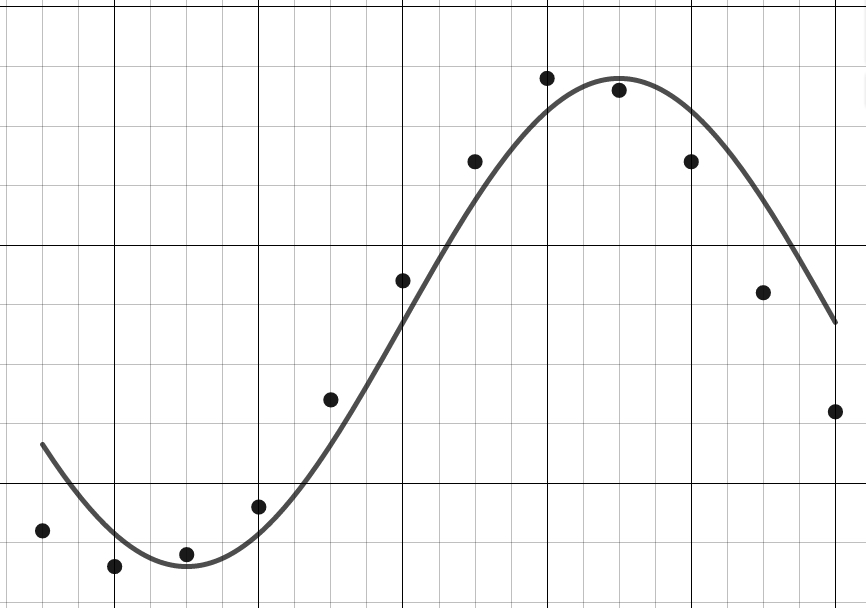
\includegraphics[height=1.5in]{./GraphsofSineandCosineGraphics/LakeErieTempReg.jpg} 

\end{center}

\item The average temperature on April $15^{\text{th}}$ is approximately $T(4.5) \approx 39.00^{\circ}$F and the average temperature on September $15^{\text{th}}$ is approximately $T(9.5) \approx 73.38^{\circ}$F.

\item  Desmos gives: $T(t) = 20.8374 \sin (-0.5251 t-0.2812) +52.3659$.  


\begin{center}

 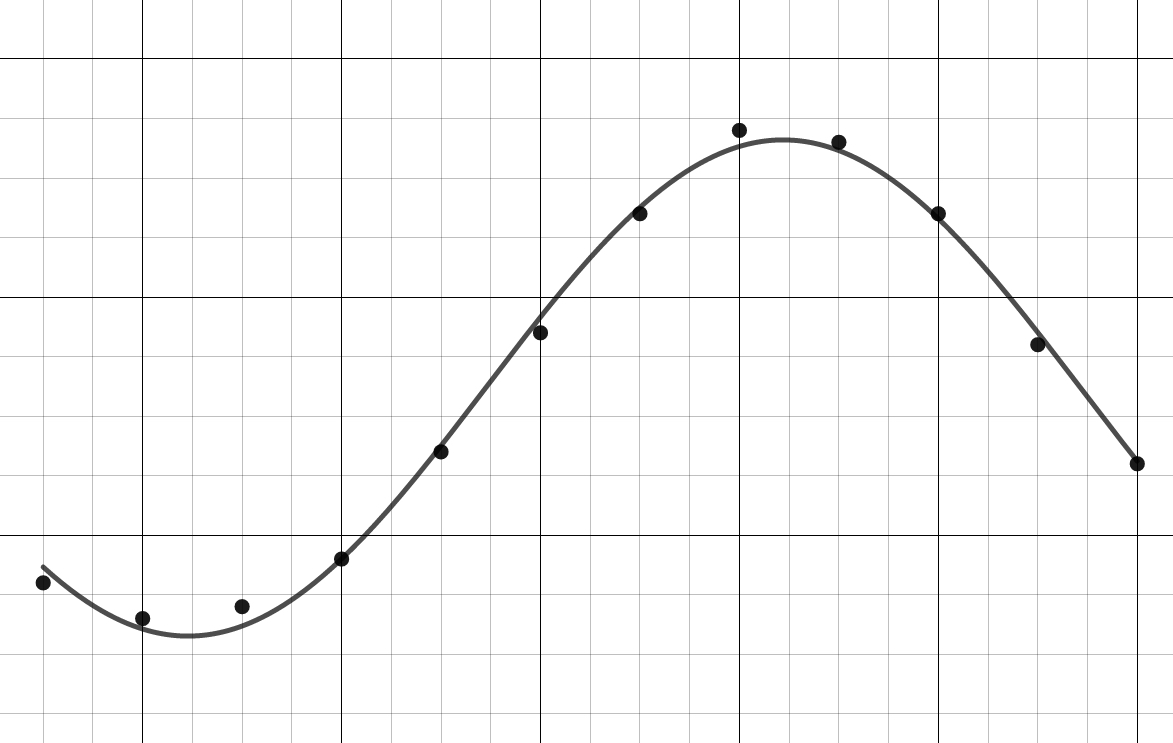
\includegraphics[height=1.5in]{./GraphsofSineandCosineGraphics/LakeErieRegDesmos.jpg} 

\end{center}

This model predicts the average temperature for April $15^{\text{th}}$ to be approximately $42.42^{\circ}$F and the average temperature on September $15^{\text{th}}$ to be approximately $70.05^{\circ}$F.  This model appears to be more accurate.

\end{enumerate}


\item  \begin{enumerate} \item  Based on the shape of the data, we either choose $A<0$ or we find the \textit{second} value of $t$ which closely approximates the `baseline' value, $F = 0.505$.  We choose the latter to obtain $F(t) = 0.475 \sin\left(\frac{\pi}{15} t - 2\pi \right) + 0.505 =  0.475 \sin\left(\frac{\pi}{15} t\right) + 0.505$ 

\enlargethispage{\baselineskip}

\item  Our function and the data set are graphed below.  It's a pretty good fit.

\begin{center}

 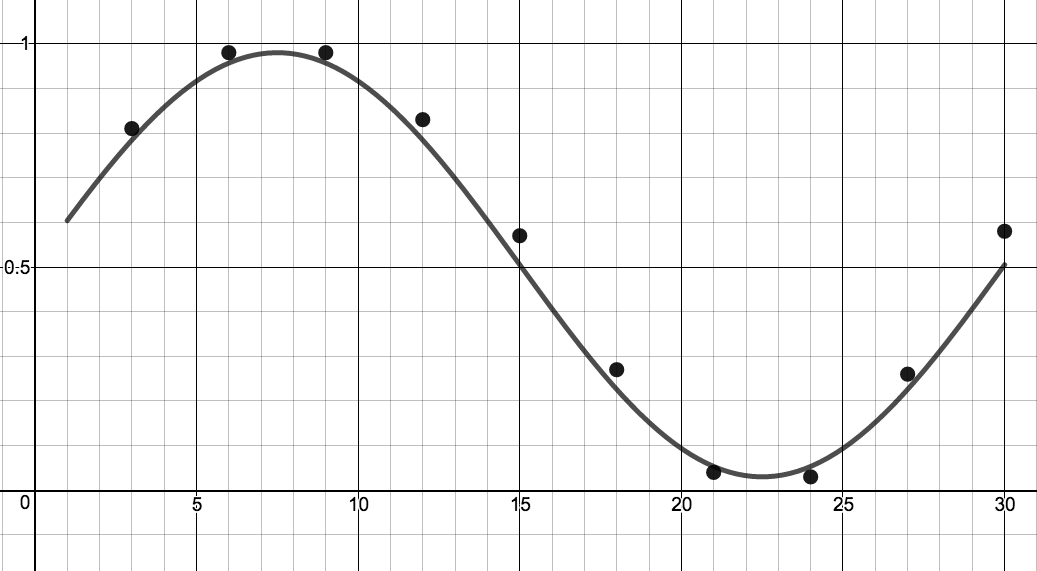
\includegraphics[height=1.5in]{./GraphsofSineandCosineGraphics/MoonIlluminationReg.jpg} 

\end{center}


\item  The fraction of the moon illuminated on June 1st, 2009 is approximately $F(1) \approx 0.60$


\item  Using desmos,\footnote{\ldots specifying $\omega = \frac{\pi}{15}$ \ldots} we get $F(t) = 0.49\sin \left(\frac{\pi }{15}t-6.29\right)+0.535$.

\begin{center}

 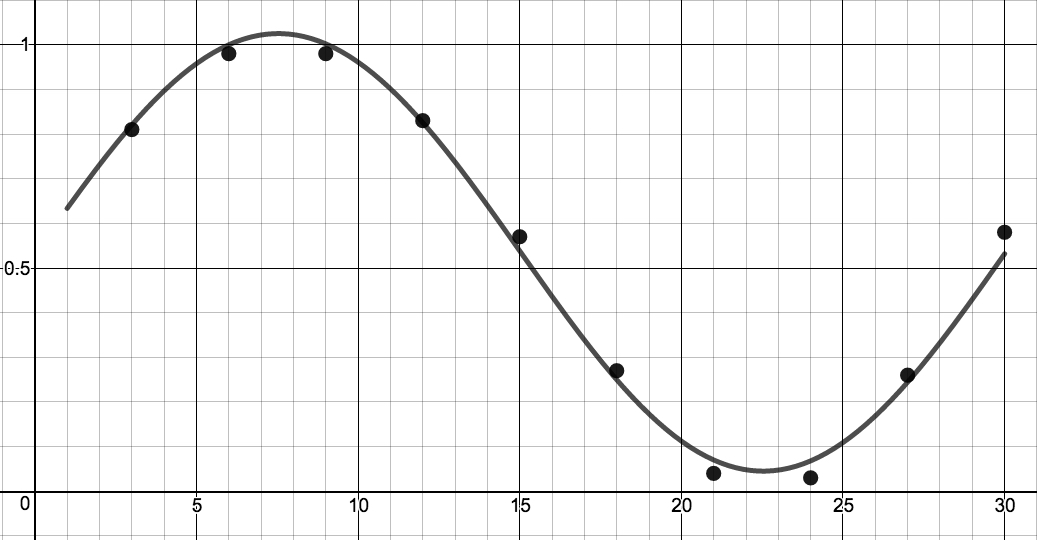
\includegraphics[height=1.5in]{./GraphsofSineandCosineGraphics/MoonIlluminatonDesmos.jpg} 

\end{center}

This model predicts that the fraction of the moon illuminated on June 1st, 2009 is approximately $0.63$.  This appears to be a better fit to the data than our first model.

\end{enumerate}


\end{enumerate}




